\documentclass[14pt]{article}
\usepackage{layout} 
% Affiche les marges des pages
\usepackage[T1]{fontenc}
\usepackage[french]{babel}
\usepackage[]{tikz}
\usepackage[document]{ragged2e}
\usepackage{times}
\usepackage[utf8]{inputenc}
\usepackage{systeme}
\usepackage{hyphenat}
\usepackage{geometry}

\usepackage{enumerate}
 \geometry{
    a4paper,
    total={170mm,257mm},
    left=20mm,
    right=15mm, 
    top=10mm
}
 \usepackage{lscape}
 \usepackage{xcolor}
 \usepackage{tkz-tab}
% Affiche les marges des pages
\linespread {1.2} % Interlines
\setlength{\parindent}{4em}
\setlength{\parskip}{1em}
\renewcommand{\baselinestretch}{2.0}
\usepackage{longtable}
\reversemarginpar
\vspace{.2in}
\usepackage{tikz}
% \usepackage{pgfplots}
% \pgfplotsset{compat = newest}
\usepackage{fancyhdr}
\pagestyle{fancy}
\usepackage{amsmath}
\usepackage{amsfonts}
\usepackage{tabularx}
\usepackage{amssymb}
\usepackage{physics}
\usepackage{siunitx}[=2021-04-09]
\usepackage{setspace}
\doublespacing
\usetikzlibrary{arrows,positioning,shapes,fit,calc}
\usepackage{hyperref}
\hypersetup{
    colorlinks=true,
    linkcolor=blue,
    filecolor=magenta,      
    urlcolor=cyan,
    pdftitle={Overleaf Example},
    pdfpagemode=FullScreen,
    }
    \usepackage{graphicx}
\graphicspath{images/}

\graphicspath{{\subfix{../images/}}} 

\usepackage{blindtext}
\usepackage{subfiles} % Best loaded last in the preamble

\title{ Commencé le 20.12.2021 \\ TM Experience de JJ Thomson}
\author{Mejda  }
\date{18 janvier 2022}

\begin{document}

\maketitle
%\begin{figure}[bh] 
 %       \centering
  %      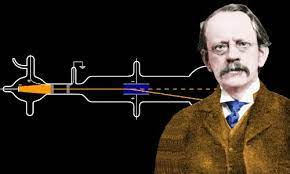
\includegraphics[width=4cm]{00.JJ-THOMSON-TUBE} 
  %      \includegraphics[width=4cm]{00.JJ-THOMSON-LAB-WIDE}
  %      \includegraphics[width=4cm]{01.JJ-THOMSON-LAB-THIN}
  %      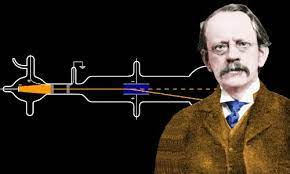
\includegraphics[width=4cm]{00.JJ-THOMSON}
  %      \label{fig:img1}
  %      \caption{Lived 1856 – 1940. }
  %  \end{figure}
\subfile{sections/03.plan_TM}
%\subfile{sections/06.texte_livre_chimie}
%\subfile{sections/livre_physique}
\end{document}
